% fig13_pr_roll — UFO capstone PRs grouped by phase.
% Standalone pgfplots; compiled to figures/fig13_pr_roll.pdf.
% Comparison (PR count by phase) => chart (commons comparison rule).
% Data: Appendix K, companion/pr-roll.json:
%   verify ladder (V1-V4) 4, pipeline (C: spec, verify) 2, sibling (CERN) 1,
%   monograph (this) 1.
\documentclass[border=4pt]{standalone}
\usepackage{tikz}
\usepackage{pgfplots}
\pgfplotsset{compat=1.18}
\begin{document}
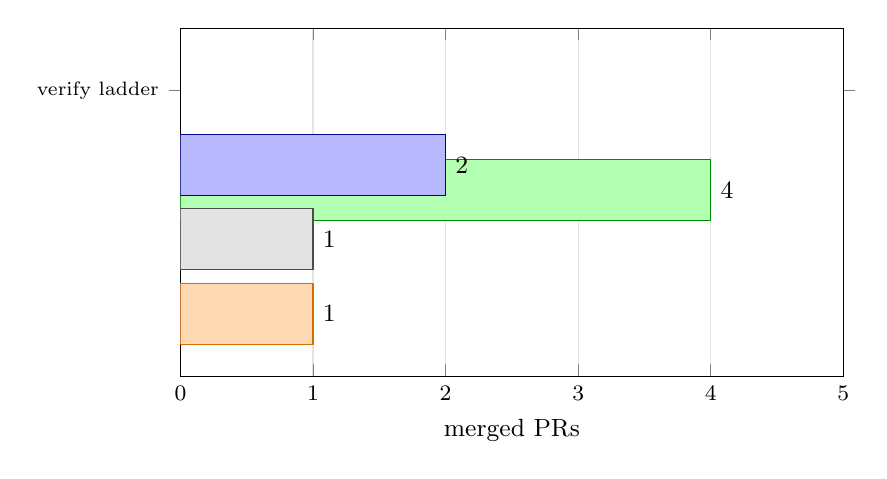
\begin{tikzpicture}
\begin{axis}[
  width=10cm, height=6.0cm,
  xbar,
  bar width=22pt,
  xmin=0, xmax=5,
  xlabel={merged PRs},
  symbolic y coords={{monograph (this)}, {sibling (CERN)}, {pipeline (C)}, {verify ladder}},
  ytick=data,
  y tick label style={font=\scriptsize},
  tick label style={font=\footnotesize},
  label style={font=\small},
  nodes near coords,
  nodes near coords style={font=\small},
  xmajorgrids, grid style={gray!22},
  enlarge y limits=0.28,
]
\addplot[draw=green!55!black,fill=green!30] coordinates {(4,{verify ladder})};
\addplot[draw=blue!55!black,fill=blue!28, bar shift=0pt] coordinates {(2,{pipeline (C)})};
\addplot[draw=gray!60!black,fill=gray!22, bar shift=0pt] coordinates {(1,{sibling (CERN)})};
\addplot[draw=orange!85!black,fill=orange!30, bar shift=0pt] coordinates {(1,{monograph (this)})};
\end{axis}
\end{tikzpicture}
\end{document}
